%----------------------------------------------------------------------------------------
% Preambulo y Configuración
%----------------------------------------------------------------------------------------

\documentclass[
    11pt,
    spanish,
    singlespacing,
    parskip,
    headsepline,
    bookmarks=true,
    unicode=true,
    pdftoolbar=true,
    pdfmenubar=true,
    pdffitwindow=false,
    colorlinks=true,
    linkcolor=blue,
    citecolor=blue,
    urlcolor=blue
]{MastersDoctoralThesis}

\usepackage[utf8]{inputenc} % Codificación de entrada UTF-8
\usepackage[T1]{fontenc}    % Codificación de salida para caracteres especiales
\usepackage{graphicx}       % Manejo de gráficos
\usepackage{eso-pic}        % Permite agregar fondos
\usepackage{hyperref}       % Manejo de hipervínculos y marcadores

% Redefinición de caracteres problemáticos en marcadores
\hypersetup{
    pdftitle={Título del Documento},
    pdfauthor={Autor del Documento},
    pdfkeywords={Sistemas Embebidos, Internet de las Cosas, Inteligencia Artificial},
    pdfstartview={FitH},
    unicode=true,
    colorlinks=true,
    linkcolor=blue,
    citecolor=blue,
    urlcolor=blue
}

\pdfstringdefDisableCommands{%
  \def\texttt#1{#1}%
  \def\textbf#1{#1}%
  \def\textit#1{#1}%
  \def\"{\"}%
  \def\~{~}%
  \def\'{'}%
  \def\^{}%
  \def\textunderscore{\_} % Manejo del subrayado en marcadores
}


% Definir comandos requeridos por la clase
\newcommand{\degreename}{Ing} % Cambia según tu título
\newcommand{\univname}{Universidad Nacional de Ejemplo} % Cambia según tu universidad
\newcommand{\keywordnames}{Palabras clave:}
%----------------------------------------------------------------------------------------
% Documento Principal
%----------------------------------------------------------------------------------------

\begin{document}

% Configuración de la portada
\posgrado{Carrera / Maestría}
\keywords{Sistemas Embebidos, Internet de las Cosas, Inteligencia Artificial}

% Incluir la portada desde un archivo separado
%----------------------------------------------------------------------------------------
% PORTADA
%----------------------------------------------------------------------------------------
\begin{titlepage}
    % Fondo completo con el PDF que incluye la barra y el logo
    \AddToShipoutPictureBG*{
\includegraphics[width=\paperwidth, height=\paperheight]{Figures/fondo.pdf}}

    % Contenido principal
    \begin{flushright}
        \setlength{\rightskip}{-2cm} % Ajusta la sangría derecha
        \vspace*{7.5cm} % Ajustar según la posición vertical deseada

        % Título
        {\fontfamily{phv}\bfseries\fontsize{33pt}{40pt}\selectfont
        Sistema de monitoreo de \textit{Rhynchophorus Ferrugineus} en palmeras de la ciudad de Montevideo} \\[1.5cm]

        % Autor
        {\fontfamily{phv}\fontsize{20pt}{25pt}\selectfont
        Ing. Bruno Masoller} \\[1cm]

        % Carrera o Maestría (comentar o descomentar la línea correspondiente)
        {\fontfamily{phv}\fontsize{15pt}{20pt}\selectfont
            % \textbf{Carrera de Especialización en Sistemas Embebidos}
            % \textbf{Carrera de Especialización en Internet de las Cosas} \\
            \textbf{Carrera de Especialización en Inteligencia Artificial}
            % \textbf{Maestría en Sistemas Embebidos} \\
            % \textbf{Maestría en Internet de las Cosas} \\
            % \textbf{Maestría en Inteligencia Artificial Embebida} \\
            % \textbf{Maestría en Computación de Borde} \\
            % \textbf{Maestría en Inteligencia Artificial} \\
        } \\[2cm]

        % Director
        {\fontfamily{phv}\fontsize{11pt}{15pt}\selectfont
        \textbf{Director:} Ing. Juan Ignacio Cavalieri (FIUBA)} \\[1cm]

        % Jurados
        {\fontfamily{phv}\fontsize{11pt}{15pt}\selectfont
        \textbf{Jurados:}} \\[0.5cm]
        {\fontfamily{phv}\fontsize{11pt}{15pt}\selectfont
        Jurado 1 (pertenencia)} \\ 
        {\fontfamily{phv}\fontsize{11pt}{15pt}\selectfont
        Jurado 2 (pertenencia)} \\ 
        {\fontfamily{phv}\fontsize{11pt}{15pt}\selectfont
        Jurado 3 (pertenencia)} \\[2cm]

        % Fecha y lugar
        {\fontfamily{phv}\itshape\fontsize{10pt}{12pt}\selectfont
        Ciudad de Montevideo, junio de 2025} % Ejemplo: Ciudad de Córdoba, junio de 2025
        % TODO: Cambiar la fecha según corresponda
    \end{flushright}
\end{titlepage}


% Configuración del contenido preliminar
\frontmatter % Usar numeración romana para las páginas preliminares
\pagestyle{plain} % Estilo de encabezado simple

%----------------------------------------------------------------------------------------
% Resumen
%----------------------------------------------------------------------------------------

\begin{abstract}
\addchaptertocentry{\abstractname} % Agregar resumen al índice
Esta memora describe la implementación de una plataforma para la intendencia de Montevideo que utiliza visión por computadora para detectar la plaga del picudo rojo en las palmeras esta ciudad. El sistema se desarrolló con el objetivo de reducir costos operativos y mejorar la toma de decisiones para el servicio de arbolado de la institución.

Para el desarrollo del trabajo fueron necesarios los conocimientos de visión por computadora, análisis de datos y aprendizaje profundo, así como de despliegue y operaciones de modelos de aprendizaje de máquinas e infraestructura de soporte.						
\end{abstract}

%----------------------------------------------------------------------------------------
% Agradecimientos
%----------------------------------------------------------------------------------------

\begin{acknowledgements}
\vspace{1.5cm}
Esta sección es para agradecimientos personales y es totalmente \textbf{OPCIONAL}.
\end{acknowledgements}

%----------------------------------------------------------------------------------------
% Índice
%----------------------------------------------------------------------------------------

\tableofcontents
\listoffigures
\listoftables

%----------------------------------------------------------------------------------------
% Dedicatoria
%----------------------------------------------------------------------------------------

\dedicatory{\textbf{Dedicado a... [OPCIONAL]}}

%----------------------------------------------------------------------------------------
% Capítulos
%----------------------------------------------------------------------------------------

\mainmatter % Iniciar numeración numérica para el contenido principal
\pagestyle{thesis} % Estilo de encabezado de tesis

% Incluir capítulos desde archivos separados
% Chapter 1

\chapter{Introducción general} % Main chapter title

\label{Chapter1} % For referencing the chapter elsewhere, use \ref{Chapter1} 
\label{IntroGeneral}

En este capítulo se presenta una introducción general al trabajo realizado. Se describe el problema que el \textit{Rhynchophorus Ferrugineus} (picudo rojo) presenta en las palmeras de la ciudad de Montevideo, el estado del arte en cuanto a trabajos similares y los objetivos planteados por la Intendencia de Montevideo (IM) y por el equipo de trabajo.

%--------------------------------------------------------------------------------------------------------------------------------------------------------------------------------

% Define some commands to keep the formatting separated from the content 
\newcommand{\keyword}[1]{\textbf{#1}}
\newcommand{\tabhead}[1]{\textbf{#1}}
\newcommand{\code}[1]{\texttt{#1}}
\newcommand{\file}[1]{\texttt{\bfseries#1}}
\newcommand{\option}[1]{\texttt{\itshape#1}}
\newcommand{\grados}{$^{\circ}$}
\newcommand{\comment}[1]{}

%--------------------------------------------------------------------------------------------------------------------------------------------------------------------------------
\section{Descripción del problema}
\label{sec:descProblema}

El picudo rojo, que puede observarse en la figura \ref{fig:picudo-rojo}, es un insecto que afecta a las palmeras, especialmente a la \textit{Phoenix Canariensis}, que es la especie más común en Montevideo. Este insecto ha causado un daño significativo en la flora de la ciudad, lo que ha llevado a la IM a enfocarse en su control y erradicación.

\begin{figure}[htpb]
  \centering
  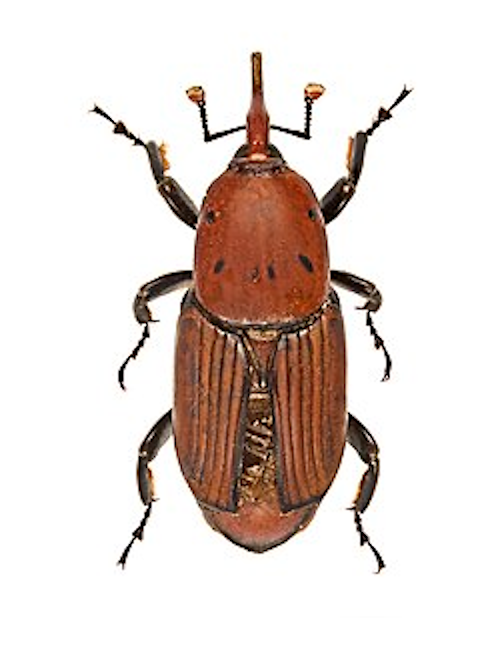
\includegraphics[scale=1]{./Figures/picudo-rojo.png}
  \caption{Picudo rojo \protect\footnotemark.}
  \label{fig:picudo-rojo}
\end{figure}

\footnotetext{Imagen tomada de \url{https://es.wikipedia.org/wiki/Rhynchophorus_ferrugineus}}

Este escarabajo supone una amenaza grave para las palmeras infectadas ya que las larvas de este insecto se alimentan del tejido interno de la planta, causando su colapso estructural en un período de meses (dado el corto corto ciclo de vida del picudo rojo \citep{anticimex_picudo_nodate}), como puede verse en la figura \ref{fig:palmera-infectada}. Esta amenaza aumenta según la época del año, puesto que el insecto tiene diferentes tasas de dispersión y reproducción dependiendo de la temperatura y la humedad. Existen varios tipos de picudos \citep{poplin_palm_2014}, algunos autóctonos y otros introducidos.

La plaga del picudo rojo llegó a Uruguay en 2022 \citep{mgap_informacion_nodate}, y se esparció rápidamente por la ciudad de Montevideo. De las 25 000 palmeras que forman una parte esencial de la ciudad, muchas ya han sucumbido a la plaga, donde se estima que para el año 2030 el ecosistema se verá ampliamente afectado \citep{arcos_picudo_2024} si no se toman medidas de control adecuadas. Últimamente también se ha esparcido por el interior del país, como puede observarse en la figura \ref{fig:palmeras-ruta5}, perteneciente a la ruta 5 de Uruguay, donde se han encontrado palmeras muertas por la plaga.

\begin{figure}[htpb]
  \centering
  \begin{subfigure}[b]{0.49\textwidth}
    \centering
    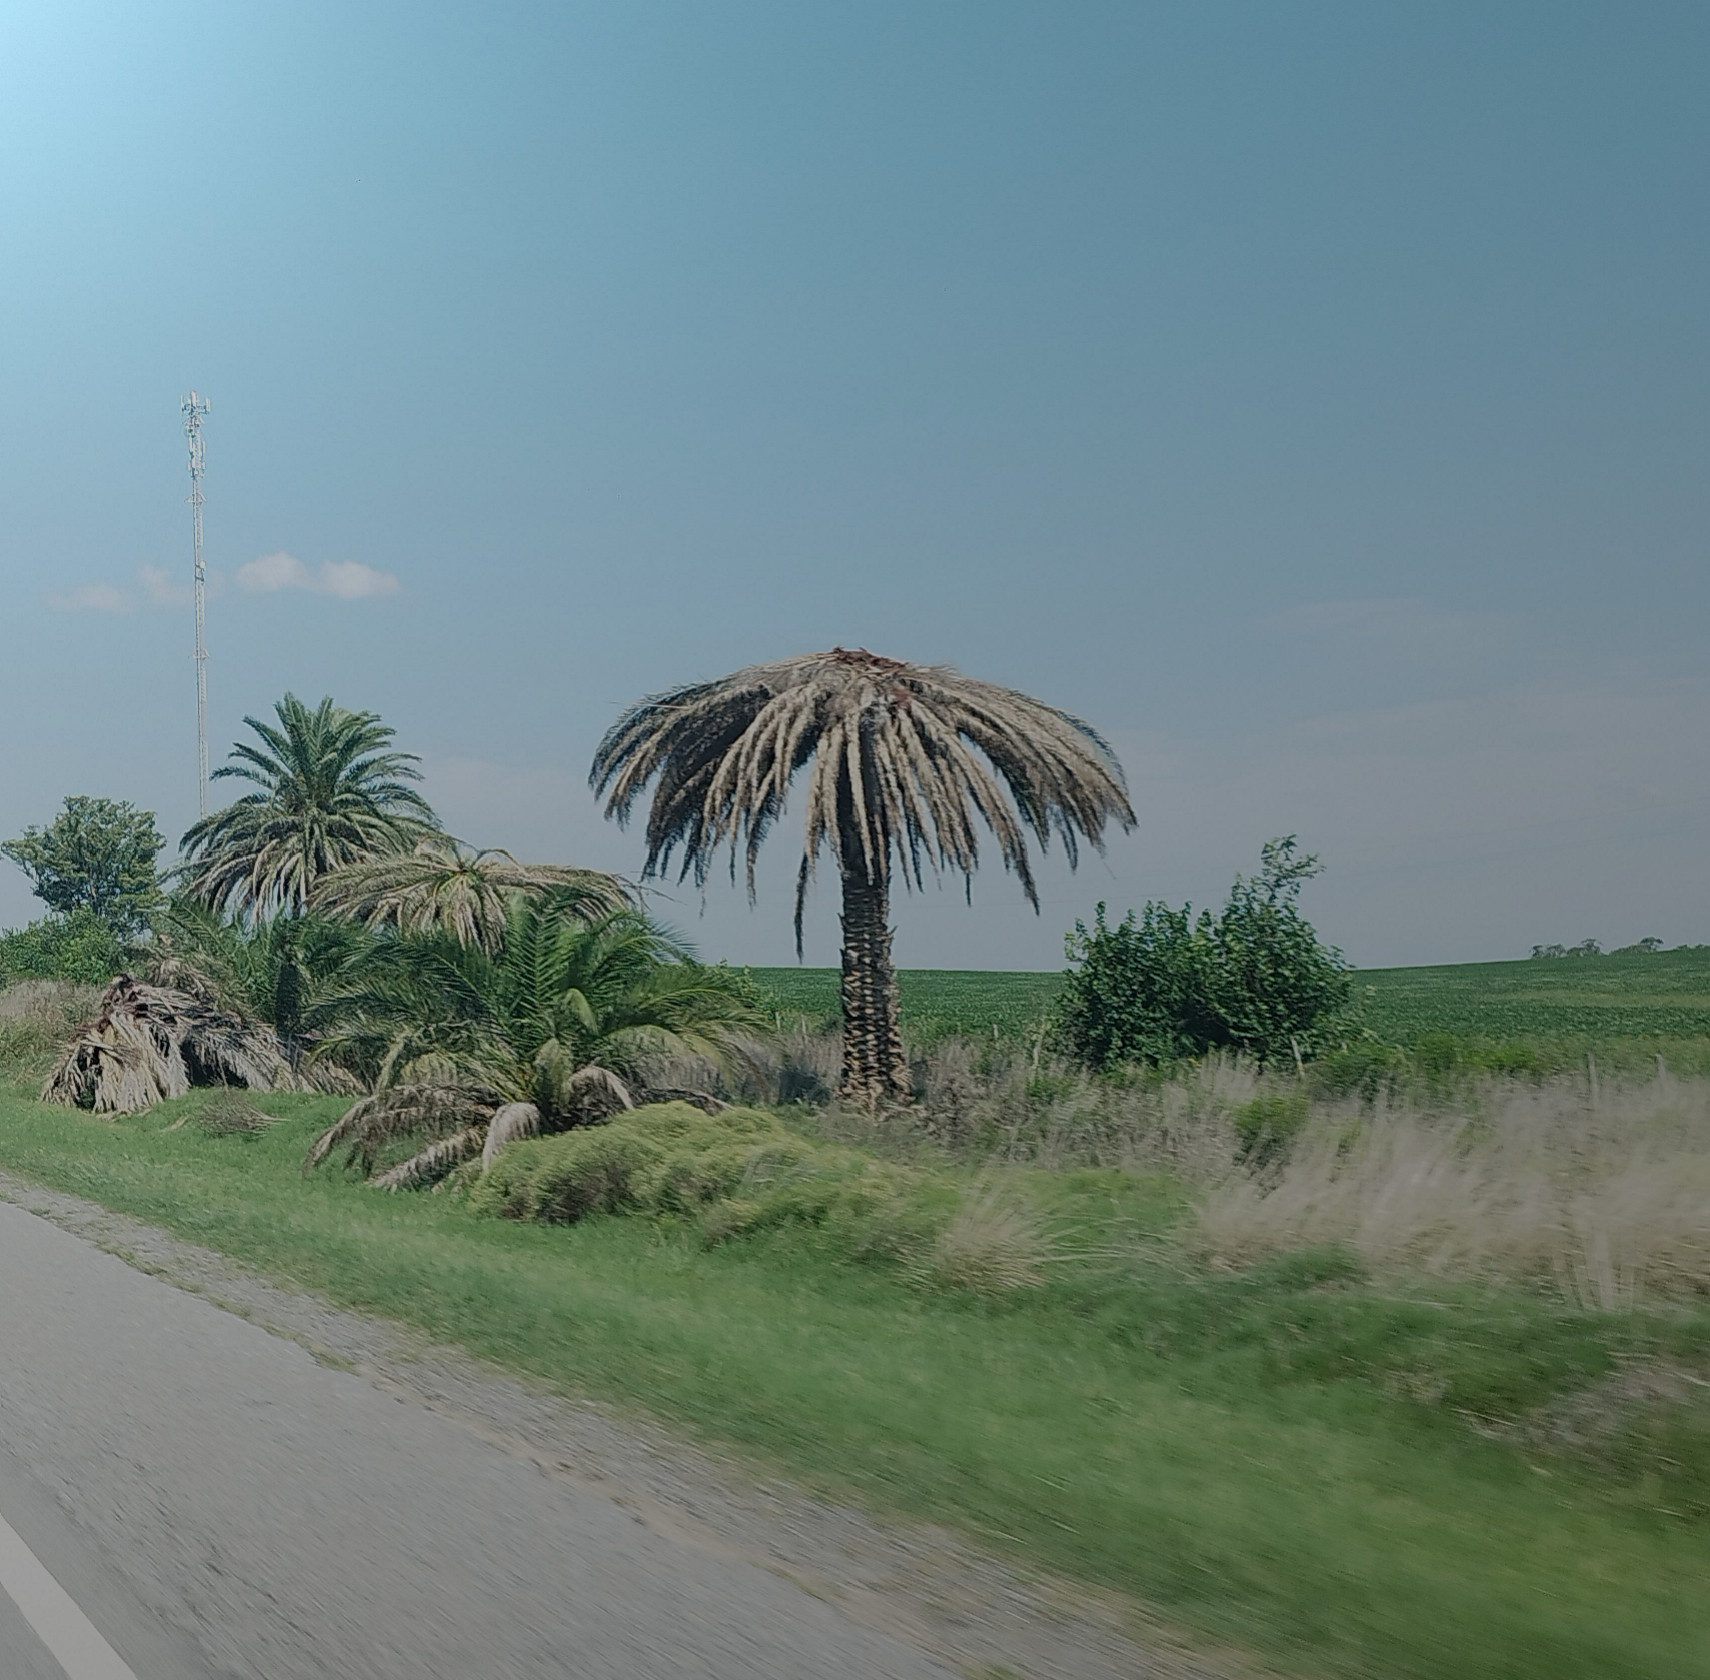
\includegraphics[width=\textwidth]{./Figures/palmera-infectada.jpg}
    \caption{Palmera infectada por el picudo rojo.}
    \label{fig:palmera-infectada}
  \end{subfigure}
  \hfill
  \begin{subfigure}[b]{0.49\textwidth}
    \centering
    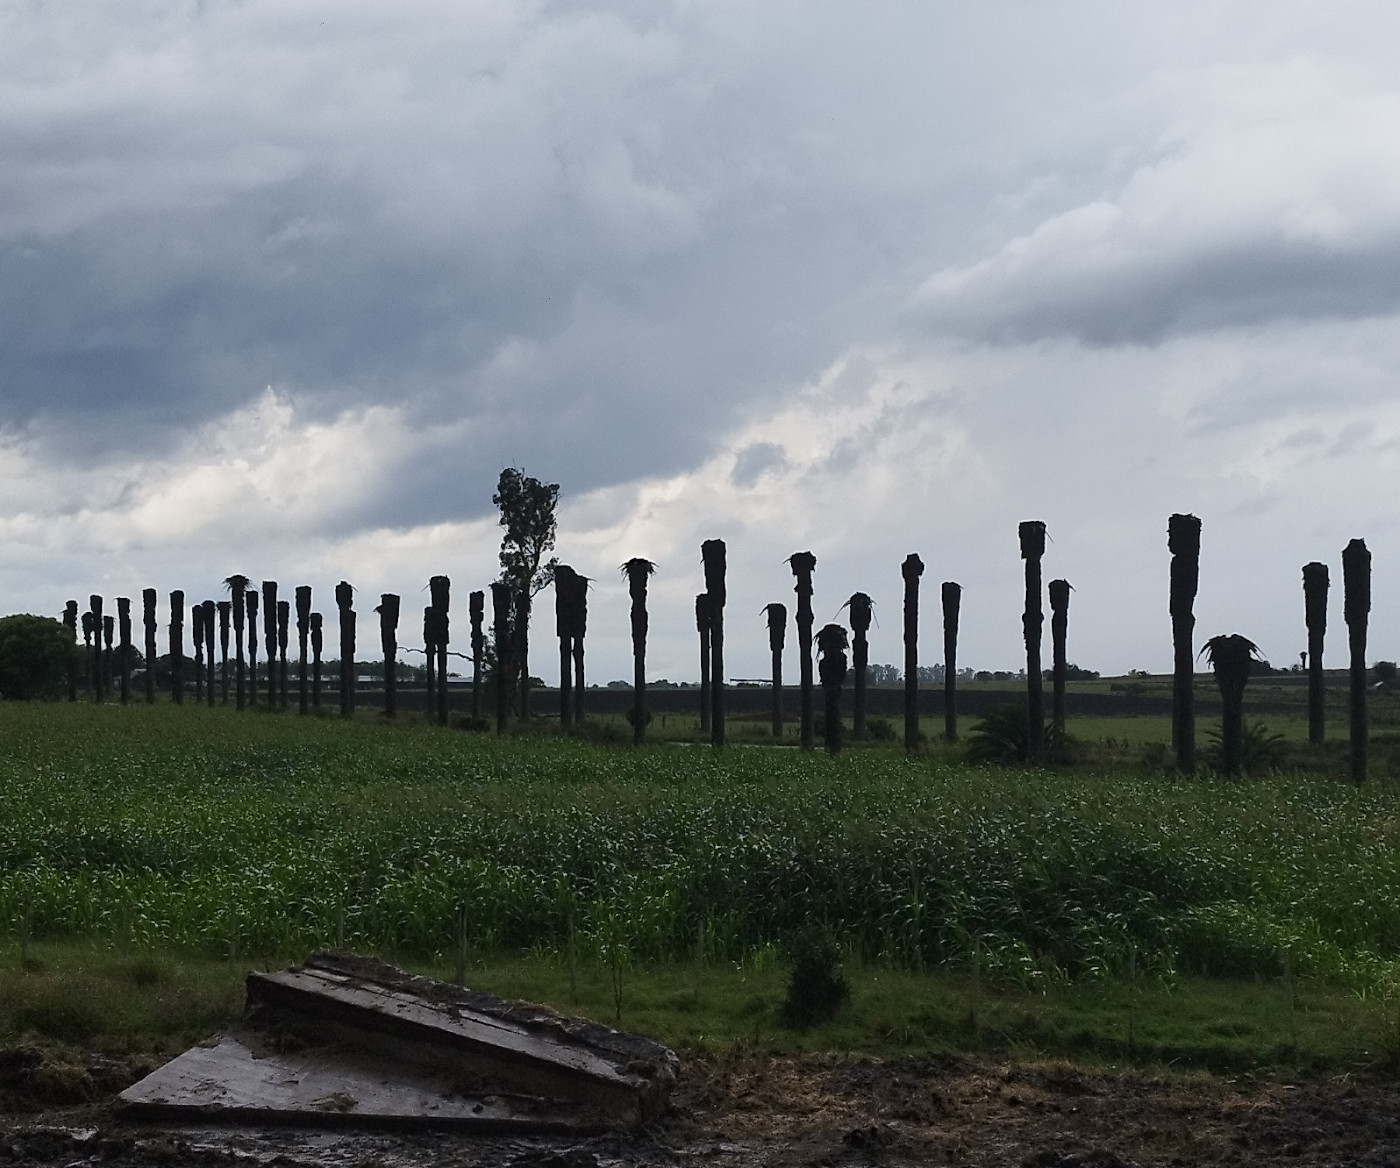
\includegraphics[width=.99\textwidth]{./Figures/palmeras-ruta5.jpg}
    \caption{Palmeras muertas en la ruta 5 de Uruguay.}
    \label{fig:palmeras-ruta5}
  \end{subfigure}
  \caption{Infección y muerte de palmeras por el picudo rojo.}
  \label{fig:infeccion-y-muerte-palmeras}
\end{figure}

Entre los métodos de control fitosanitarios que se utilizan para combatir la plaga se encuentran la endoterapia \citep{intendencia_de_montevideo_acciones_nodate}, el baño, la cirugía \citep{sanchez_cirugiespecializada_nodate} y la remoción. Sin embargo, estos métodos son costosos y requieren de un monitoreo constante para detectar la presencia del picudo rojo. Para la IM no es solamente una cuestión ecológica sino también económica. En este sentido, el servicio de arbolado realiza un seguimiento de las palmeras afectadas por la plaga. Para ello, se registra su ubicación y estado de salud mediante campañas de detecciones a pie. Este proceso manual requiere de mucho tiempo y recursos humanos, por lo que resulta imprescindible un sistema automatizado que permita detectar la presencia de la plaga en lugares específicos de Montevideo.

Uno de los recursos aún no explotados por la IM para el monitoreo de la plaga es el uso de imágenes aéreas obtenidas mediante drones, disponibles por el servicio de geomática de ésta institución. Estos ortomosaicos, que pueden observarse en la figura \ref{fig:ejemplo-ortomosaico}, permiten obtener información detallada sobre el estado de las palmeras y su entorno.

\begin{figure}[H]
  \centering
  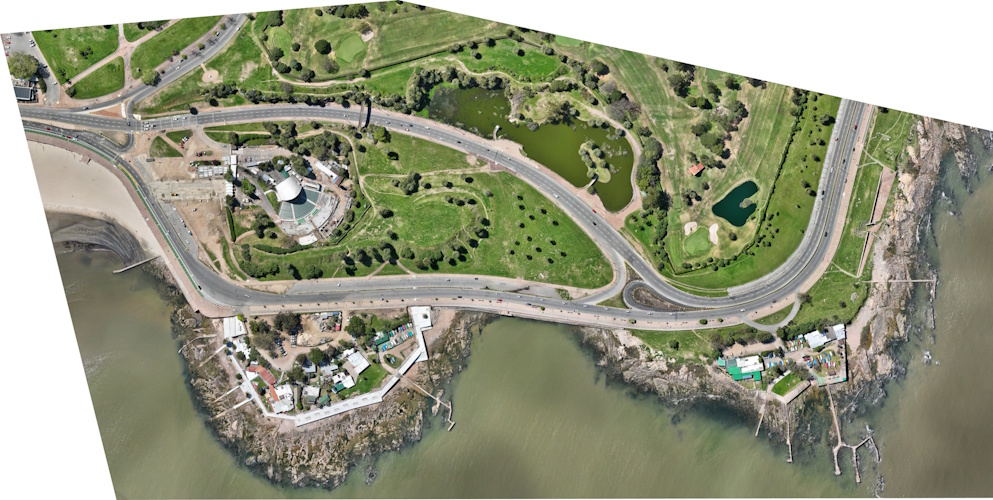
\includegraphics[scale=0.5]{./Figures/ejemplo-ortomosaico.jpg}
  \caption{Ejemplo de ortomosaico \protect\footnotemark.}
  \label{fig:ejemplo-ortomosaico}
\end{figure}

\footnotetext{Imagen tomada del sistema de información geográfica de la IM (SIG): \url{https://sig.montevideo.gub.uy/}}

El análisis de estas imágenes es un proceso complejo que requiere de técnicas avanzadas de procesamiento de imágenes y aprendizaje automático, así como también herramientas que brinden soporte a estas actividades.

%--------------------------------------------------------------------------------------------------------------------------------------------------------------------------------
\section{Estado del arte}
\label{sec:estadoArte}

En los últimos años, el campo de la visión por computadora (VPC) ha experimentado un crecimiento exponencial, impulsado principalmente por los avances en el aprendizaje profundo y las redes neuronales convolucionales (CNN, por su sigla en inglés de \textit{Convolutional Neural Networks}). Estas tecnologías han permitido el desarrollo de soluciones innovadoras para tareas de detección, clasificación y segmentación en imágenes, lo que ha abierto nuevas posibilidades para aplicaciones en diversos ámbitos, tales como la monitorización ambiental y la agricultura de precisión. La detección de plagas mediante imágenes aéreas, en particular la del picudo rojo, ha cobrado relevancia debido al creciente impacto que este insecto tiene en la salud de las palmeras urbanas, principalmente en países del Mediterráneo y en el Medio Oriente \citep{poplin_palm_2014}.
En esta sección se revisan las principales técnicas y enfoques que han marcado el estado del arte en la detección de plagas a partir de imágenes aéreas. Se aborda tanto arquitecturas tradicionales como las más recientes, donde se destacan sus fortalezas, limitaciones y la evolución de sus aplicaciones en escenarios reales.

\subsection{Redes convolucionales}
\label{sec:redesConvolucionales}

La visión por computadora abarca una amplia gama de tareas, tales como la detección de objetos, la segmentación de imágenes, el reconocimiento de patrones y la clasificación de imágenes. Estas tareas suelen abordarse mediante modelos de CNN. Tendencias recientes evidencian avances significativos en el diseño de estas redes para el procesamiento de imágenes. En particular, se ha puesto énfasis en el tratamiento de imágenes de alta resolución capturadas mediante vehículos aéreos no tripulados (UAV, por su sigla en inglés de \textit{Unmanned Aerial Vehicles}), lo que representa un área de aplicación de creciente interés del sector académico y privado \citep{gao_recent_2024} \citep{sutar_convolutional_2025}.

\subsection{Detección del picudo rojo en imágenes aéreas}

La relevancia de la detección de la plaga del picudo rojo a nivel global ha propiciado el surgimiento de diversas líneas de investigación. En este sentido, se han desarrollado enfoques basados en VPC a partir de imágenes aéreas, haciendo especial uso de arquitecturas de CNN tales como YOLO \citep{redmon_you_2016}.

Entre los estudios analizados, la implementación de la detección mediante imágenes aéreas de forma exclusiva representa una metodología relativamente novedosa. En este contexto, en el estudio \textit{Automatic large scale detection of red palm weevil infestation using street view images} \citep{kagan_automatic_2021}, se emplea un enfoque combinado. Inicialmente, se localizan las palmeras a través de una CNN (Faster R-CNN \citep{ren_faster_2016}) aplicada a imágenes aéreas. Posteriormente, utilizando la misma arquitectura, se extrae la corona de la palmera a partir de imágenes capturadas en \textit{street view}, lo que permite clasificar a la planta en función de la presencia o ausencia de infección. Un resumen de este trabajo se presenta en la figura \ref{fig:kagan-automatic-2021-process}.

\begin{figure}[htpb]
  \centering
  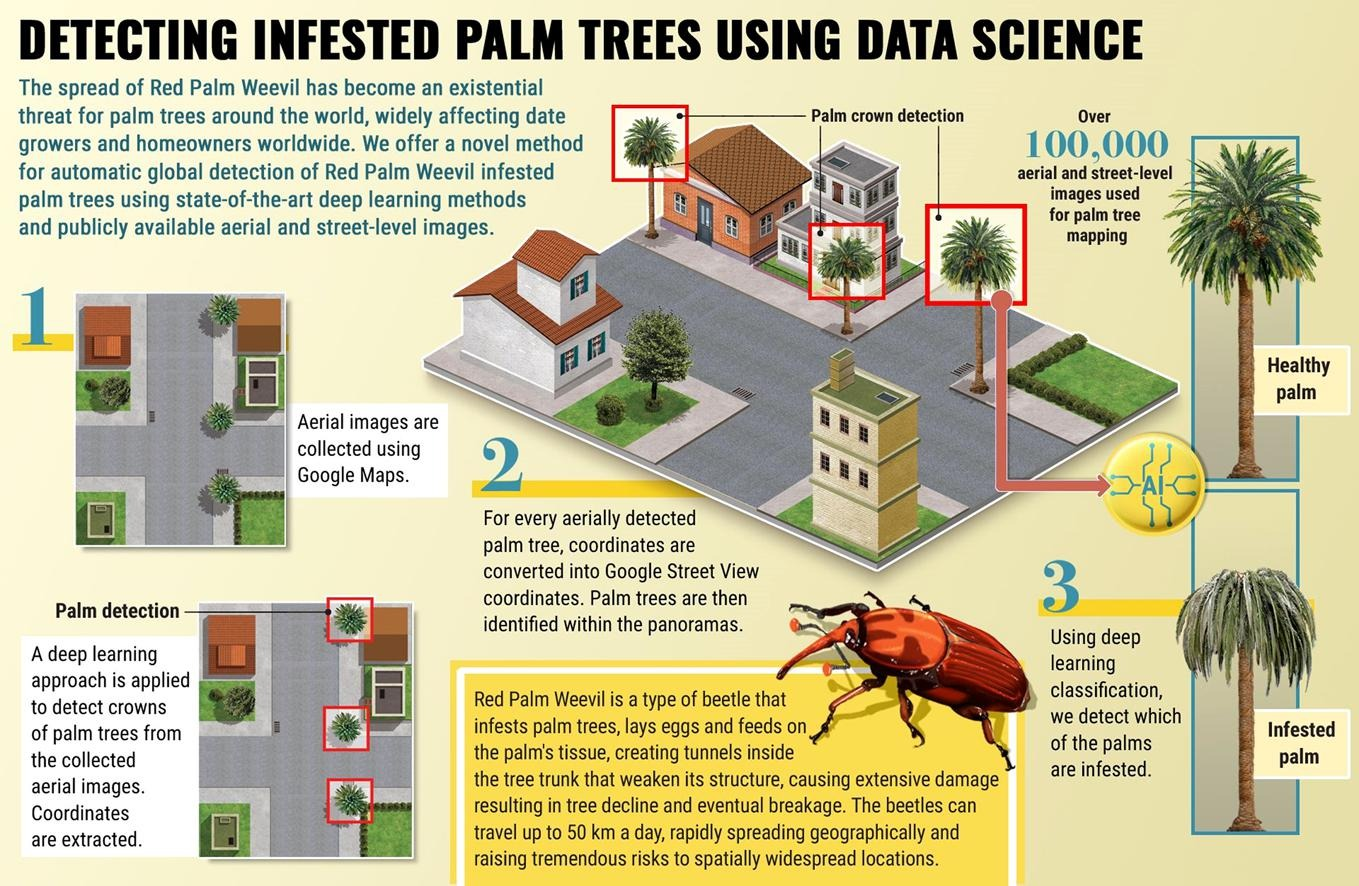
\includegraphics[scale=1.8]{./Figures/kagan_automatic_2021-process.jpg}
  \caption{Proceso de detección realizado por Kagan et al \protect\footnotemark.}
  \label{fig:kagan-automatic-2021-process}
\end{figure}

\footnotetext{Imagen obtenida de: \url{http://arxiv.org/abs/1506.01497}}

Por otro lado, la detección de palmeras sí es ampliamente estudiada en la literatura, siendo un tema recurrente en la investigación de VPC. En este sentido, se han desarrollado diversos estudios. En \textit{Implementation of slicing aided hyper inference (SAHI) in YOLOv8 to counting oul palm trees using high-resolution aereal imagery data} \citep{zhorif_implementation_2024} se presenta un enfoque que utiliza la arquitectura YOLOv8 para detectar palmeras en imágenes aéreas de alta resolución. Además, utiliza \textit{Slicing Aided Hyper Inference} para mejorar la precisión de la detección. Este enfoque se basa en la idea de dividir las imágenes en regiones más pequeñas y realizar inferencias en cada una de ellas, lo que permite una detección más precisa de los objetos de interés, algo esencial en el caso de objetos pequeños como las palmeras. Para el estudio, se utilizaron imágenes RGB capturadas con un dron Trinity F90+ a 200 metros de altura y una implementación de segmentación (SAHI) de \SI{3000}{}\,\texttimes\,\SI{3000}{\pixel}. Si bien el estudio se centra en la detección de palmeras de aceite, su metodología puede ser adaptada para la detección del picudo rojo. La tabla \ref{tab:papers-deteccion-palmeras} resume los métodos utilizados en la detección de palmeras en diferentes estudios anteriores.

\begin{table}[H]
  \centering
  \caption[Comparación entre diferentes estudios de detección de palmeras]{Comparación entre diferentes estudios de detección de palmeras \footnotemark.}
  \begin{tabular}{{l c c}}
    % \begin{tabular}{{l p{4cm} p{4cm}}}
    \toprule
    \textbf{Autor y año}                                               & \textbf{Modelo}       & \textbf{Métricas}                 \\
    \midrule
    Mukhles Sir Monea et al, 2022 \citep{muna_development_2023}        & YOLOv3                & 5.76\% (MAPE)                     \\
    Hery Wibowo et al, 2022 \citep{wibowo_large-scale_2022}            & \makecell[c]{YOLOv3,                                      \\YOLOv4, \\YOLOv5m}            & \makecell[c]{97.28\% (v3), \\97.74\% (v4), \\94.94\% (v5m). \\(F1-Score)}              \\
    Adel Ammar et al, 2022 \citep{ammar_deep-learning-based_2021}      & Faster R-CNN          & \makecell[c]{94.99\% (Precision), \\84\% (Recall), \\83\% (AP IoU)}                 \\
    Wardana et al, 2023 \citep{wardana_detection_2023}                 & YOLOv8                & 98.50\% (Overall Accuracy)        \\
    Deta Sandya Prasitha et al, 2022 \citep{prasvita_automatic_nodate} & \makecell[c]{YOLOv5s,                                     \\YOLOv5m, \\YOLOv5l, \\YOLOv5x} & \makecell[c]{0.82 (v5s), \\0.84 (v5m), \\0.85 (v5l), \\0.86 (v5x). \\(Average F1-Score)} \\
    Nuwar et al, 2022 \citep{nuwara_modern_2022}                       & YOLOv5                & 0.895 (F1-Score)                  \\
    Junos et al, 2022 \citep{junos_notitle_nodate}                     & YOLOv3n               & \makecell[c]{97.20\% (mAP),       \\0.91 (F1-Score)}                                     \\
    \bottomrule
    \hline
  \end{tabular}
  \label{tab:papers-deteccion-palmeras}
\end{table}

% \begin{table}[h]
%   \centering
%   \caption[comparativa-papers]{Comparación entre diferentes estudios de detección de palmeras\footnotemark.}
%   \begin{adjustbox}{width=\textwidth}
%     \begin{tabular}{l c c}
%       \toprule
%       \textbf{Author and Year}         & \textbf{Method}                    & \textbf{Evaluation}                                                \\
%       \midrule
%       Mukhles Sir Monea et al, 2022    & YOLOv3                             & 5.76\% (MAPE)                                                      \\
%       Hery Wibowo et al, 2022          & YOLOv3, YOLOv4, YOLOv5m            & 97.28\% (v3), 97.74\% (v4), 94.94\% (v5m). (F1-Score)              \\
%       Adel Ammar et al, 2022           & Faster R-CNN                       & 94.99\% (Precision), 84\% (Recall), 83\% (AP IoU)                  \\
%       Wardana et al, 2023              & YOLOv8                             & 98.50\% (Overall Accuracy)                                         \\
%       Deta Sandya Prasitha et al, 2022 & YOLOv5s, YOLOv5m, YOLOv5l, YOLOv5x & 0.82 (v5s), 0.84 (v5m), 0.85 (v5l), 0.86 (v5x). (Average F1-Score) \\
%       Nuwar et al, 2022                & YOLOv5                             & 0.895 (F1-Score)                                                   \\
%       Junos et al, 2022                & YOLOv3n                            & 97.20\% (mAP), 0.91 (F1-Score)                                     \\
%       \bottomrule
%       \hline
%     \end{tabular}
%   \end{adjustbox}
%   \label{}
% \end{table}

\footnotetext{Tabla obtenida de \textit{Implementation of slicing aided hyper inference (SAHI) in YOLOv8 to counting oul palm trees using high-resolution aereal imagery data} \citep{zhorif_implementation_2024}}

También, se han realizado estudios controlados como en \textit{Red Palm Weevil Detection in Date Palm Using Temporal UAV Imagery} \citep{delalieux_red_2023}, en donde se concluye que la detección del picudo rojo es posible mediante imágenes aéreas en el rango infrarrojo.

%--------------------------------------------------------------------------------------------------------------------------------------------------------------------------------

\section{Objetivos y alcance}
\label{sec:objetivos}

La finalidad principal del presente trabajo consistió en validar una prueba de concepto para la detección del picudo rojo en palmeras de Montevideo, utilizando imágenes aéreas capturadas mediante drones. Con este objetivo, se desarrolló un sistema fundamentado en técnicas de VPC y aprendizaje profundo, que permite identificar la presencia de la plaga. Para ello, se utilizó la información centralizada en el SIG \citep{intendencia_de_montevideo_sistema_nodate}, complementado con herramientas adicionales que facilitaron la generación del conjunto de datos de entrenamiento.

Adicionalmente, se planteó ante la IM la necesidad de optimizar los procesos de detección de la plaga, con miras a una mejora en la asignación de recursos humanos y económicos. El alcance inicial se centró exclusivamente en la detección del picudo rojo. En los capítulos siguientes se detalla tanto la descripción de las herramientas utilizadas como el proceso metodológico implementado.
\chapter{Introducción específica} % Main chapter title

\label{Chapter2}

%----------------------------------------------------------------------------------------
%	SECTION 1
%----------------------------------------------------------------------------------------
Todos los capítulos deben comenzar con un breve párrafo introductorio que indique cuál es el contenido que se encontrará al leerlo.  La redacción sobre el contenido de la memoria debe hacerse en presente y todo lo referido al proyecto en pasado, siempre de modo impersonal.

\section{Estilo y convenciones}
\label{sec:ejemplo}

\subsection{Uso de mayúscula inicial para los título de secciones}

Si en el texto se hace alusión a diferentes partes del trabajo referirse a ellas como capítulo, sección o subsección según corresponda. Por ejemplo: ``En el capítulo \ref{Chapter1} se explica tal cosa'', o ``En la sección \ref{sec:ejemplo} se presenta lo que sea'', o ``En la subsección \ref{subsec:ejemplo} se discute otra cosa''.

Cuando se quiere poner una lista tabulada, se hace así:

\begin{itemize}
	\item Este es el primer elemento de la lista.
	\item Este es el segundo elemento de la lista.
\end{itemize}

Notar el uso de las mayúsculas y el punto al final de cada elemento.

Si se desea poner una lista numerada el formato es este:

\begin{enumerate}
	\item Este es el primer elemento de la lista.
	\item Este es el segundo elemento de la lista.
\end{enumerate}

Notar el uso de las mayúsculas y el punto al final de cada elemento.

\subsection{Este es el título de una subsección}
\label{subsec:ejemplo}

Se recomienda no utilizar \textbf{texto en negritas} en ningún párrafo, ni tampoco texto \underline{subrayado}. En cambio sí se debe utilizar \textit{texto en itálicas} para palabras en un idioma extranjero, al menos la primera vez que aparecen en el texto. En el caso de palabras que estamos inventando se deben utilizar ``comillas'', así como también para citas textuales. Por ejemplo, un \textit{digital filter} es una especie de ``selector'' que permite separar ciertos componentes armónicos en particular.

La escritura debe ser impersonal. Por ejemplo, no utilizar ``el diseño del firmware lo hice de acuerdo con tal principio'', sino ``el firmware fue diseñado utilizando tal principio''. 

El trabajo es algo que al momento de escribir la memoria se supone que ya está concluido, entonces todo lo que se refiera a hacer el trabajo se narra en tiempo pasado, porque es algo que ya ocurrió. Por ejemplo, "se diseñó el firmware empleando la técnica de test driven development".

En cambio, la memoria es algo que está vivo cada vez que el lector la lee. Por eso transcurre siempre en tiempo presente, como por ejemplo:

``En el presente capítulo se da una visión global sobre las distintas pruebas realizadas y los resultados obtenidos. Se explica el modo en que fueron llevados a cabo los test unitarios y las pruebas del sistema''.

Se recomienda no utilizar una sección de glosario sino colocar la descripción de las abreviaturas como parte del mismo cuerpo del texto. Por ejemplo, RTOS (\textit{Real Time Operating System}, Sistema Operativo de Tiempo Real) o en caso de considerarlo apropiado mediante notas a pie de página.

Si se desea indicar alguna página web utilizar el siguiente formato de referencias bibliográficas, dónde las referencias se detallan en la sección de bibliografía de la memoria, utilizado el formato establecido por IEEE en \citep{IEEE:citation}. Por ejemplo, ``el presente trabajo se basa en la plataforma EDU-CIAA-NXP \citep{CIAA}, la cual...''.

\subsection{Figuras} 

Al insertar figuras en la memoria se deben considerar determinadas pautas. Para empezar, usar siempre tipografía claramente legible. Luego, tener claro que \textbf{es incorrecto} escribir por ejemplo esto: ``El diseño elegido es un cuadrado, como se ve en la siguiente figura:''

\begin{figure}[h]
\centering

\includegraphics[scale=.45]{./Figures/cuadradoAzul.png}
\end{figure}

La forma correcta de utilizar una figura es con referencias cruzadas, por ejemplo: ``Se eligió utilizar un cuadrado azul para el logo, como puede observarse en la figura \ref{fig:cuadradoAzul}''.

\begin{figure}[ht]
	\centering
	
\includegraphics[scale=.45]{./Figures/cuadradoAzul.png}
	\caption{Ilustración del cuadrado azul que se eligió para el diseño del logo.}
	\label{fig:cuadradoAzul}
\end{figure}

El texto de las figuras debe estar siempre en español, excepto que se decida reproducir una figura original tomada de alguna referencia. En ese caso la referencia de la cual se tomó la figura debe ser indicada en el epígrafe de la figura e incluida como una nota al pie, como se ilustra en la figura \ref{fig:palabraIngles}.

\begin{figure}[htpb]
	\centering
	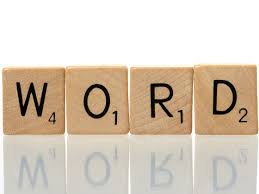
\includegraphics[scale=.3]{./Figures/word.jpeg}
	\caption{Imagen tomada de la página oficial del procesador\protect\footnotemark.}
	\label{fig:palabraIngles}
\end{figure}

\footnotetext{Imagen tomada de \url{https://goo.gl/images/i7C70w}}

La figura y el epígrafe deben conformar una unidad cuyo significado principal pueda ser comprendido por el lector sin necesidad de leer el cuerpo central de la memoria. Para eso es necesario que el epígrafe sea todo lo detallado que corresponda y si en la figura se utilizan abreviaturas entonces aclarar su significado en el epígrafe o en la misma figura.



\begin{figure}[ht]
	\centering
	
\includegraphics[scale=.37]{./Figures/questionMark.png}
	\caption{¿Por qué de pronto aparece esta figura?}
	\label{fig:questionMark}
\end{figure}

Nunca colocar una figura en el documento antes de hacer la primera referencia a ella, como se ilustra con la figura \ref{fig:questionMark}, porque sino el lector no comprenderá por qué de pronto aparece la figura en el documento, lo que distraerá su atención.

Otra posibilidad es utilizar el entorno \textit{subfigure} para incluir más de una figura, como se puede ver en la figura \ref{fig:three graphs}. Notar que se pueden referenciar también las figuras internas individualmente de esta manera: \ref{fig:1de3}, \ref{fig:2de3} y \ref{fig:3de3}.
 
\begin{figure}[!htpb]
     \centering
     \begin{subfigure}[b]{0.3\textwidth}
         \centering
         
\includegraphics[width=.65\textwidth]{./Figures/questionMark}
         \caption{Un caption.}
         \label{fig:1de3}
     \end{subfigure}
     \hfill
     \begin{subfigure}[b]{0.3\textwidth}
         \centering
         
\includegraphics[width=.65\textwidth]{./Figures/questionMark}
         \caption{Otro.}
         \label{fig:2de3}
     \end{subfigure}
     \hfill
     \begin{subfigure}[b]{0.3\textwidth}
         \centering
         
\includegraphics[width=.65\textwidth]{./Figures/questionMark}
         \caption{Y otro más.}
         \label{fig:3de3}
     \end{subfigure}
        \caption{Tres gráficos simples.}
        \label{fig:three graphs}
\end{figure}

El código para generar las imágenes se encuentra disponible para su reutilización en el archivo \file{Chapter2.tex}.

\subsection{Tablas}

Para las tablas utilizar el mismo formato que para las figuras, sólo que el epígrafe se debe colocar arriba de la tabla, como se ilustra en la tabla \ref{tab:peces}. Observar que sólo algunas filas van con líneas visibles y notar el uso de las negritas para los encabezados.  La referencia se logra utilizando el comando \verb|\ref{<label>}| donde label debe estar definida dentro del entorno de la tabla.

\begin{verbatim}
\begin{table}[h]
	\centering
	\caption[caption corto]{caption largo más descriptivo}
	\begin{tabular}{l c c}    
		\toprule
		\textbf{Especie}     & \textbf{Tamaño} & \textbf{Valor}\\
		\midrule
		Amphiprion Ocellaris & 10 cm           & \$ 6.000 \\		
		Hepatus Blue Tang    & 15 cm           & \$ 7.000 \\
		Zebrasoma Xanthurus  & 12 cm           & \$ 6.800 \\
		\bottomrule
		\hline
	\end{tabular}
	\label{tab:peces}
\end{table}
\end{verbatim}


\begin{table}[h]
	\centering
	\caption[caption corto]{caption largo más descriptivo.}
	\begin{tabular}{l c c}    
		\toprule
		\textbf{Especie} 	 & \textbf{Tamaño} 		& \textbf{Valor}  \\
		\midrule
		Amphiprion Ocellaris & 10 cm 				& \$ 6.000 \\		
		Hepatus Blue Tang	 & 15 cm				& \$ 7.000 \\
		Zebrasoma Xanthurus	 & 12 cm				& \$ 6.800 \\
		\bottomrule
		\hline
	\end{tabular}
	\label{tab:peces}
\end{table}

En cada capítulo se debe reiniciar el número de conteo de las figuras y las tablas, por ejemplo, figura 2.1 o tabla 2.1, pero no se debe reiniciar el conteo en cada sección. Por suerte la plantilla se encarga de esto por nosotros.

\subsection{Ecuaciones}
\label{sec:Ecuaciones}

Al insertar ecuaciones en la memoria dentro de un entorno \textit{equation}, éstas se numeran en forma automática  y se pueden referir al igual que como se hace con las figuras y tablas, por ejemplo ver la ecuación \ref{eq:metric}.

\begin{equation}
	\label{eq:metric}
	ds^2 = c^2 dt^2 \left( \frac{d\sigma^2}{1-k\sigma^2} + \sigma^2\left[ d\theta^2 + \sin^2\theta d\phi^2 \right] \right)
\end{equation}
                                                        
Es importante tener presente que si bien las ecuaciones pueden ser referidas por su número, también es correcto utilizar los dos puntos, como por ejemplo ``la expresión matemática que describe este comportamiento es la siguiente:''

\begin{equation}
	\label{eq:schrodinger}
	\frac{\hbar^2}{2m}\nabla^2\Psi + V(\mathbf{r})\Psi = -i\hbar \frac{\partial\Psi}{\partial t}
\end{equation}

Para generar la ecuación \ref{eq:metric} se utilizó el siguiente código:

\begin{verbatim}
\begin{equation}
	\label{eq:metric}
	ds^2 = c^2 dt^2 \left( \frac{d\sigma^2}{1-k\sigma^2} + 
	\sigma^2\left[ d\theta^2 + 
	\sin^2\theta d\phi^2 \right] \right)
\end{equation}
\end{verbatim}

Y para la ecuación \ref{eq:schrodinger}:

\begin{verbatim}
\begin{equation}
	\label{eq:schrodinger}
	\frac{\hbar^2}{2m}\nabla^2\Psi + V(\mathbf{r})\Psi = 
	-i\hbar \frac{\partial\Psi}{\partial t}
\end{equation}

\end{verbatim}
\definecolor{mygreen}{rgb}{0,0.6,0}
\definecolor{mygray}{rgb}{0.5,0.5,0.5}
\definecolor{mymauve}{rgb}{0.58,0,0.82}

%%%%%%%%%%%%%%%%%%%%%%%%%%%%%%%%%%%%%%%%%%%%%%%%%%%%%%%%%%%%%%%%%%%%%%%%%%%%%
% parámetros para configurar el formato del código en los entornos lstlisting
%%%%%%%%%%%%%%%%%%%%%%%%%%%%%%%%%%%%%%%%%%%%%%%%%%%%%%%%%%%%%%%%%%%%%%%%%%%%%
\lstset{ %
  backgroundcolor=\color{white},   % choose the background color; you must add \usepackage{color} or \usepackage{xcolor}
  basicstyle=\footnotesize,        % the size of the fonts that are used for the code
  breakatwhitespace=false,         % sets if automatic breaks should only happen at whitespace
  breaklines=true,                 % sets automatic line breaking
  captionpos=b,                    % sets the caption-position to bottom
  commentstyle=\color{mygreen},    % comment style
  deletekeywords={...},            % if you want to delete keywords from the given language
  escapeinside={(*@}{@*)},          % if you want to add LaTeX within your code
  %extendedchars=true,              % lets you use non-ASCII characters; for 8-bits encodings only, does not work with UTF-8
  %frame=single,	                % adds a frame around the code
  keepspaces=true,                 % keeps spaces in text, useful for keeping indentation of code (possibly needs columns=flexible)
  keywordstyle=\color{blue},       % keyword style
  language=[ANSI]C,                % the language of the code
  %otherkeywords={*,...},           % if you want to add more keywords to the set
  numbers=left,                    % where to put the line-numbers; possible values are (none, left, right)
  numbersep=5pt,                   % how far the line-numbers are from the code
  numberstyle=\tiny\color{mygray}, % the style that is used for the line-numbers
  rulecolor=\color{black},         % if not set, the frame-color may be changed on line-breaks within not-black text (e.g. comments (green here))
  showspaces=false,                % show spaces everywhere adding particular underscores; it overrides 'showstringspaces'
  showstringspaces=false,          % underline spaces within strings only
  showtabs=false,                  % show tabs within strings adding particular underscores
  stepnumber=1,                    % the step between two line-numbers. If it's 1, each line will be numbered
  stringstyle=\color{mymauve},     % string literal style
  tabsize=2,	                   % sets default tabsize to 2 spaces
  title=\lstname,                  % show the filename of files included with \lstinputlisting; also try caption instead of title
  morecomment=[s]{/*}{*/}
}

\chapter{Diseño e implementación} % Main chapter title
\label{Chapter3} % Change X to a consecutive number; for referencing this chapter elsewhere, use \ref{ChapterX}

En este capítulo se describen los aspectos más relevantes del diseño e implementación de la plataforma. Inicialmente se presenta su arquitectura en donde se describen sus componentes e interacciones. Luego se describe el proceso de despliegue de la infraestructura de soporte, tanto en ambiente local como en ambiente de producción. Posteriormente se enfatiza la tarea de etiquetado de datos, incluyendo los problemas y soluciones enfrentados. Finalmente se presenta el entrenamiento de los modelos, seguido del despliegue e integración con el resto de la plataforma.

%----------------------------------------------------------------------------------------
%	SECTION 1
%----------------------------------------------------------------------------------------
\section{Arquitectura de la plataforma}
\label{sec:arquitectura}

El objetivo principal de este trabajo fue brindar una introducción a un sistema completo de monitoreo y detección de la plaga del picudo rojo mediante imágenes aéreas generadas por drones y/o aviones. El enfoque se basó en el módulo de VPC, donde se destacan los hitos que fueron necesarios ejecutar dentro de la IM para llevar a cabo el trabajo. Entre estos hitos se encuentra el proceso de gestión de datos, la correcta administración de los modelos de VPC y la infraestructura que soporta estos procesos. Para ello, se planteó la plataforma de la figura \ref{fig:plataforma}. Esta plataforma se basa en un enfoque modular, donde cada componente desempeña un papel específico en el proceso de detección y monitoreo de la infección.

\begin{figure}[H]
  \centering
  \includegraphics[scale=0.06]{./Figures/arquitectura-solución.png}
  \caption{Diagrama de arquitectura del sistema de monitoreo.}
  \label{fig:plataforma}
\end{figure}

El sistema se organiza en dos ecosistemas diferenciados: uno constituido por herramientas externas a la infraestructura de la IM, y otro integrado por herramientas internas.

El ecosistema externo se encarga de las interaccione con plataformas de servicios externos, como lo es Google Maps, en donde al momento de realizar el trabajo se encontraba la información relevada por el servicio de arbolado. En un futuro, esta información estaría integrada a sistemas dentro de la IM, como lo es QGIS \citep{wikipedia_qgis_2025}.

Por otra parte, en el ecosistema interno se incluyen todas las herramientas necesarias para llevar a cabo un proyecto de VPC, encapsuladas dentro de la infraestructura de la IM. Este ecosistema se basa en software de código abierto y se divide en varios módulos, lo que aumenta la sustituibilidad de piezas de software (atributo comúnmente conocido intercambiabilidad en patrones de arquitecturas de software). La comunicación se basa en protocolos ligeros como REST \citep{wikipedia_protocolo_2024}, que generan un bajo acoplamiento y una alta cohesión entre módulos. Esta plataforma cuenta también con varios módulos definidos para procesos auxiliares como la seguridad, los respaldos y la gestión de la configuración.

El módulo de seguridad permite la administración de usuarios y permisos. Esto garantiza que solo los usuarios autorizados tengan acceso a la información sensible. Este módulo se basa en el protocolo LDAP, que favorece una gestión centralizada de autenticación y autorización. Adicionalmente, el módulo puede ser sustituido por el software utilizado en la IM (WSO2 \citep{wso2_deliver_nodate}) o directamente interactuar con este (WSO2 puede comunicarse mediante el protocolo LDAP).

El módulo de respaldo de datos cerciora que los datos estén siempre disponibles y que se puedan recuperar en caso de pérdida. Gestiona procesos de respaldo y recuperación de datos, lo que mitiga riesgos asociados a la pérdida de información. Al ser un módulo independiente, puede ser sustituido por otro software de respaldo, como por ejemplo: Restic \citep{restic_restic_nodate} o Bacula \citep{bacula_documentation_nodate}.

El módulo gestor de datos es el encargado de almacenar los metadatos de las imágenes y los resultados de los modelos. Está conformado por una base de datos orientada a documentos, que permite almacenar varios tipos de datos (explicado en la sección \ref{sec:gestionRepoDatos}). Esta forma de almacenamiento, que mejora la eficiencia, facilita la gestión de grandes volúmenes de información. Asimismo, esta estructura también soluciona el desafío guardar las etiquetas generadas por los usuarios en el proceso de etiquetado de datos.

El módulo de etiquetado de datos permite ejecutar el proceso de etiquetado de imágenes y se comunica tanto con el módulo de seguridad para el manejo de diferentes niveles de información, así como con el módulo gestor de datos para almacenar las etiquetas generadas por los usuarios. Este módulo intenta estar bajamente acoplado en todo momento, por lo que la integración con repositorios de datos y proveedores de identidad es esencial para su funcionamiento.

El módulo de calidad de datos se ocupa de realizar un análisis cualitativo de los datos, lo que mejora la eficiencia de los modelos al utilizar datos de alta calidad. Este módulo permite que un equipo de control de calidad pueda analizar y generar informes específicos sobre los datos, lo que habilita una traza y evolución de lás imágenes, esencial en proyectos de VPC donde la variable temporal afecta el resultado de las predicciones, como lo es este trabajo.

El módulo de información georreferenciada permite resolver la ubicación de los elementos de interés. Esto concede que los datos estén correctamente posicionados para así emparejar las predicciones de los modelos y las coordenadas reales. Además, este módulo brinda información con mayor granularidad y un historial de los elementos, como lo son las palmeras y sus antecedentes de infección.

El módulo de repositorio de objetos es el responsable del almacenamiento y gestión de las imágenes, en este caso las generadas por drones y aviones. Este módulo administra grandes volúmenes de diferentes tipos de datos y garantiza la disponibilidad continua de esta información mediante APIs. Para esta tarea, usualmente se utilizan sistemas de almacenamiento de objetos como Amazon S3 \citep{amazon_web_services_aws_nodate} o algún otro proveedor de nube.

El módulo de aplicaciones web se encarga de gestionar la interfaz de usuarios, lo que les permite interactuar con el sistema y acceder a la información de manera sencilla. Interactúa con el sistema de información georreferenciada y muestra información sobre los elementos de interés, como las palmeras y su estado de actual de infección. También permite ingresar nueva información al sistema como nuevos focos de detección de la plaga. Esto asegura que el sistema esté actualizado en todo momento y facilita a los usuarios la visualización e identificación de estos focos.

El módulo mini-apps centraliza aplicaciones utilizadas en varias tareas, como la actualización, migración y generación de datos que usualmente son insumos para los procesos de entrenamiento. Este módulo realiza tareas específicas que no están directamente relacionadas con el proceso de detección, pero que son necesarias para el correcto funcionamiento del sistema. Un ejemplo de esto es la aplicación que efectúa \textit{web scrapping} del sistema de información geográfica de la IM, para descargar las imágenes de los vuelos allí publicadas y guardarlas en el repositorio de imágenes.

Finalmente, el módulo de IA se encarga de cumplir con los procesos asociados al entrenamiento y despliegue de los modelos. Tiene el objetivo de manejar sus el ciclos de vida, desde su desarrollo hasta su despliegue en producción. Incluye la administración de experimentos y expone una API para la interacción con otros elementos del sistema, como las aplicaciones web o las mini-apps.


La interacción entre estos componentes permite que el sistema funcione de manera eficiente y escalable. Cada módulo se encarga de una tarea específica, lo que se alinea con SRP (siglas del inglés, \textit{Single Responsibility Principle} \citep{soni_software_2024}). Esto posibilita una fácil sustitución y mejora continua del sistema. Este tipo de arquitecturas también favorece la integración de nuevas funcionalidades y la adaptación a cambios en los requisitos de la solución. Si bien el enfoque principal del trabajo fue sobre el módulo de IA, se utilizaron herramientas de soporte que satisfacen este enfoque modular, como las que se describen en la siguiente sección.

%----------------------------------------------------------------------------------------
%	SECTION 2
%----------------------------------------------------------------------------------------

\section{Despliegue de la infraestructura de soporte}
\label{sec:despliegue_infraestructura}

El despliegue de la infraestructura de soporte se llevó a cabo en dos ambientes, uno local y otro de producción.

El entorno local se utilizó para el desarrollo y la ejecución de pruebas preliminares, mientras que el de producción se destinó al despliegue final del sistema, el cual replica fielmente la infraestructura operativa de la IM.

En este contexto, el dominio local se configuró para emular el entorno de producción mediante la adopción de herramientas idénticas o análogas, tal como se ilustra en la figura \ref{fig:infra-desarrollo}.

\begin{figure}[htpb]
  \centering
  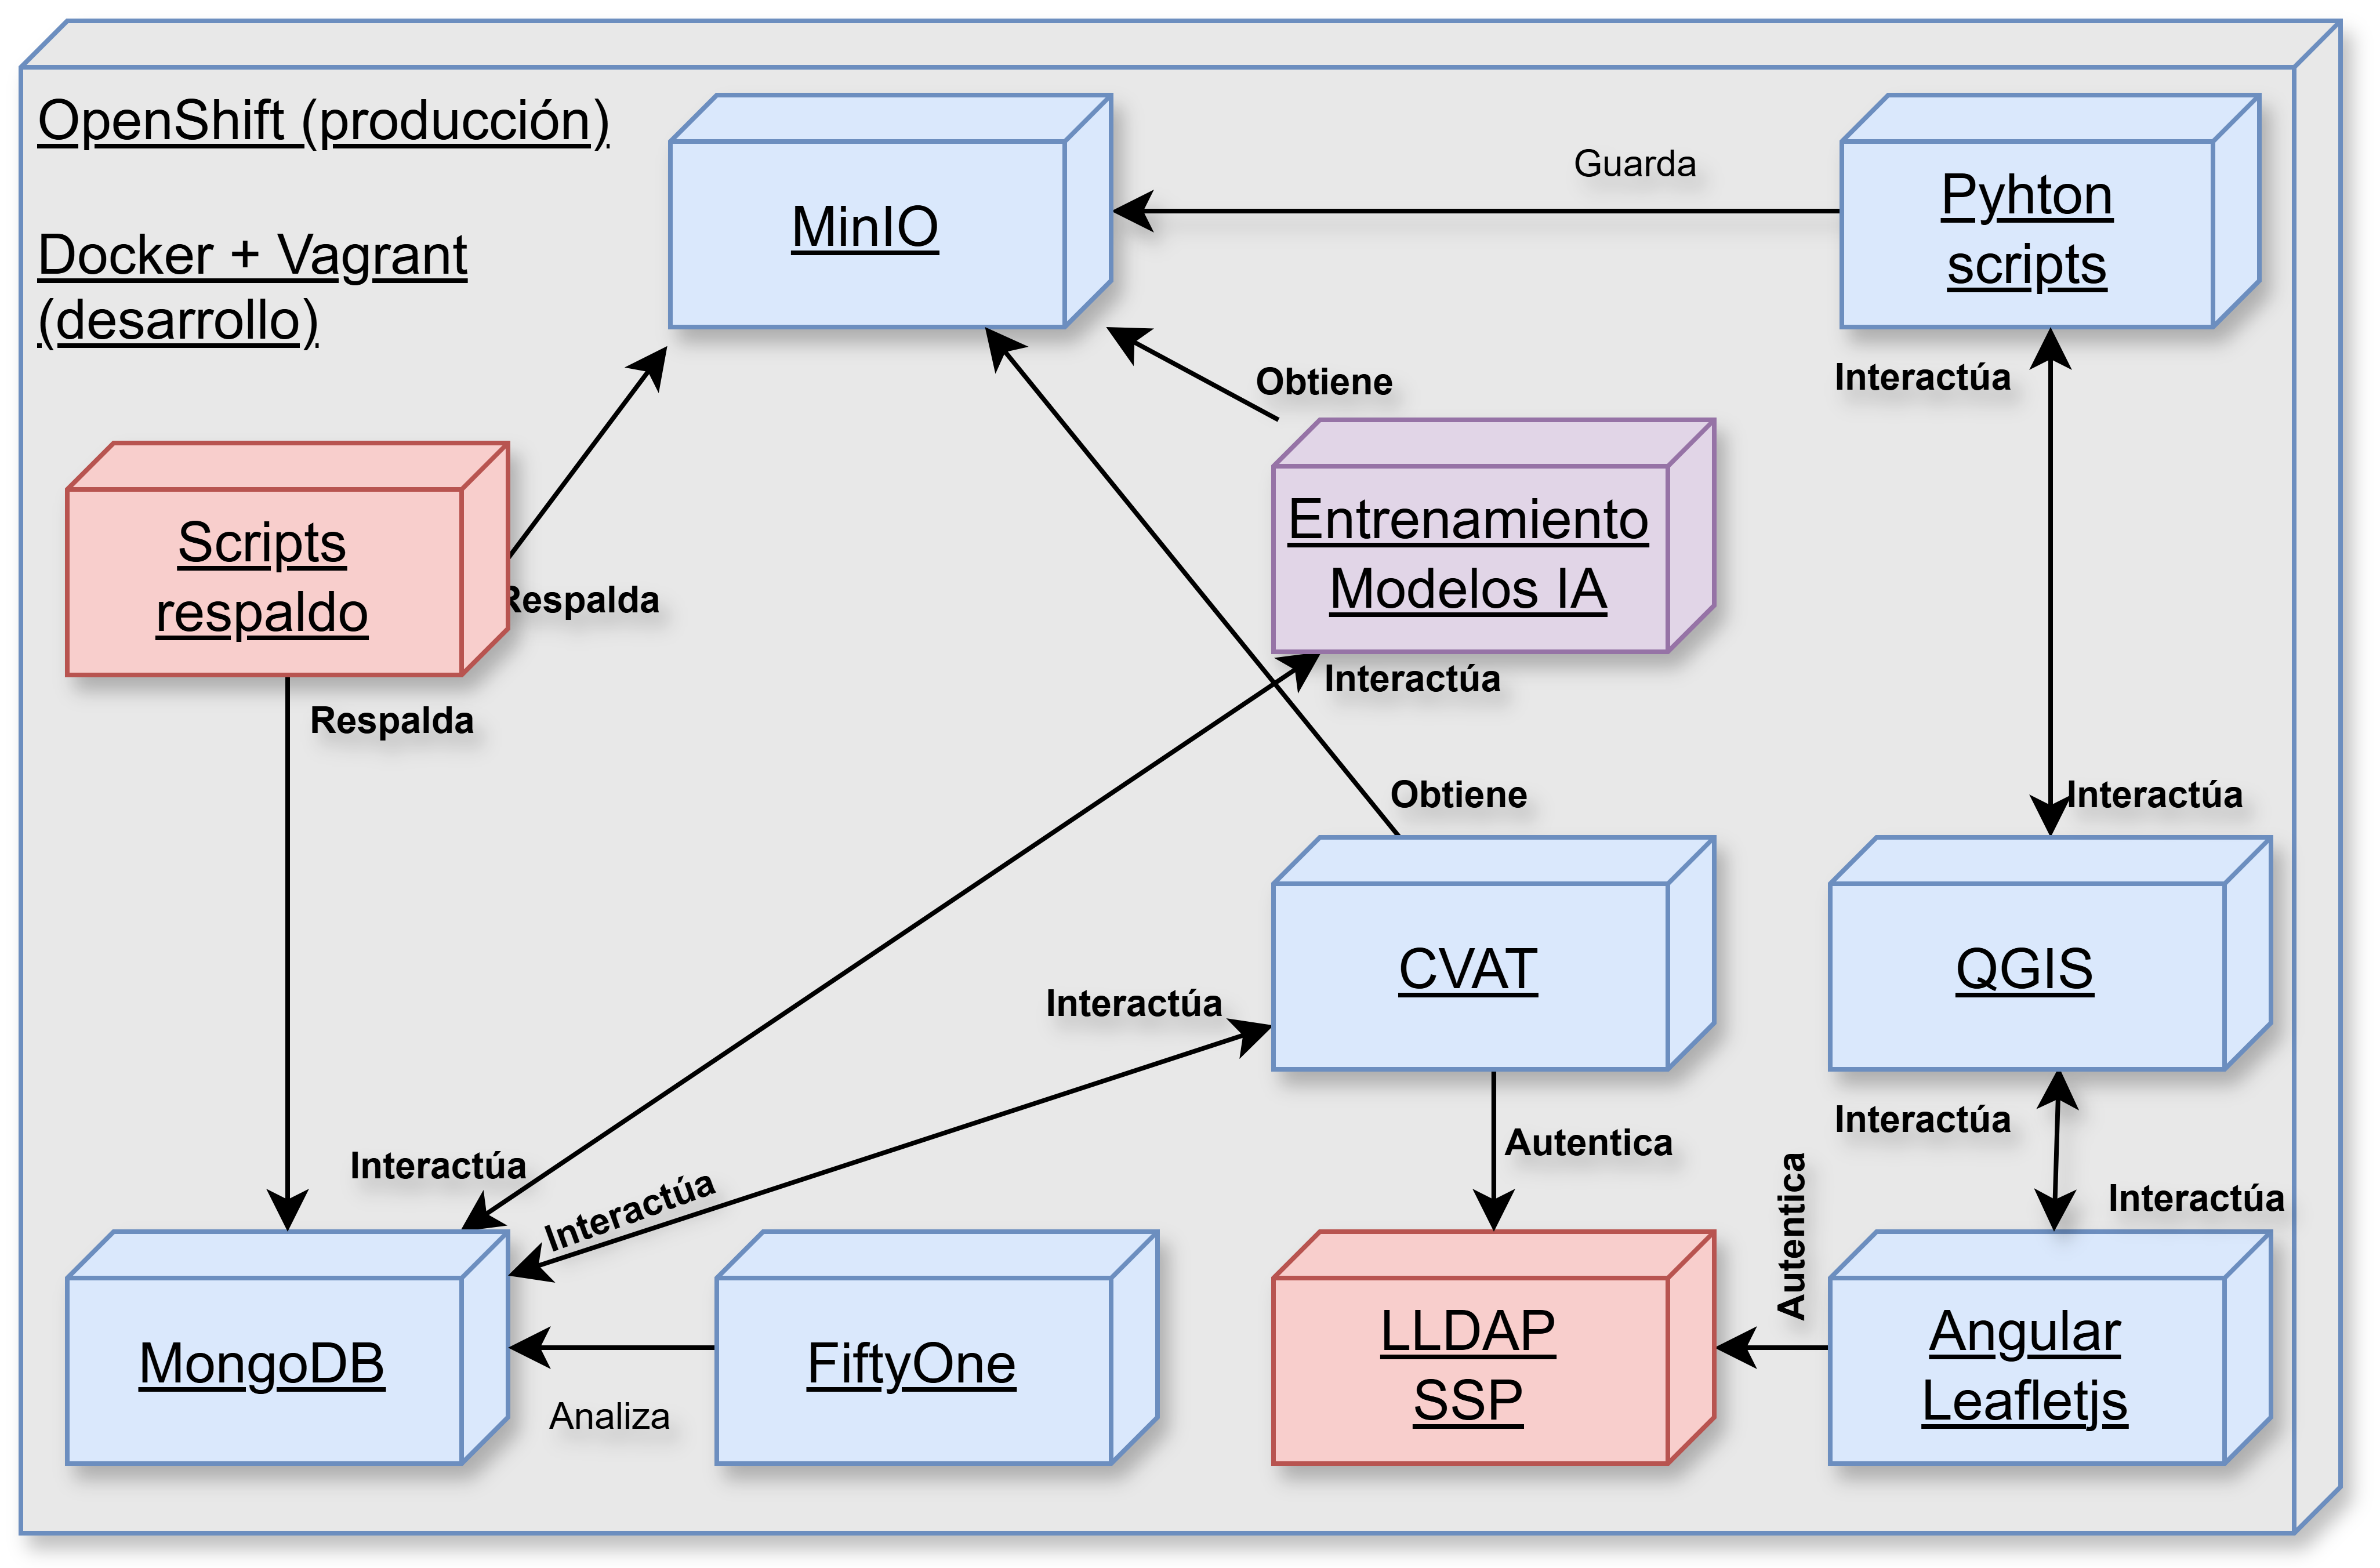
\includegraphics[scale=0.09]{./Figures/herramientas-plataforma.png}
  \caption{Diagrama de arquitectura del sistema de monitoreo.}
  \label{fig:infra-desarrollo}
\end{figure}

Otro usuario desarrollador puede tener el ambiente directamente desde su máquina, simplemente clonando el repositorio \citep{bruno_masoller_brunomaso1uba-ceia_nodate} mediante Git y luego importar el proyecto utilizando un IDE \citep{wikipedia_entorno_2025}. En este caso, se utilizó Visual Studio Code. Una vez importado el proyecto, la estructura de directorios emula cada módulo del proyecto de la siguiente manera:

% Ejemplos de código:

% \begin{lstlisting}[label=cod:vControl,caption=Estructura de directorios utilizada.]  % Start your code-block
%
%   desarrollo/
%     |-- cvat/
%
% \end{lstlisting}

% \usepackage{alltt}
% \begin{alltt}
%
%   desarrollo/
%   ├── cvat/
%
% \end{alltt}

\begin{lstlisting}[label=cod:vControl,caption=Estructura de directorios utilizada., literate={├}{{\textSFviii}}1 {─}{{\textSFx}}1 {└}{{\textSFii}}1 {│}{{\textSFxi}}1]  % Start your code-block

  desarrollo/
  ├── modulo-aplicaciones-web/
  │   ├── entrypoint/
  │   └── landing-page/
  ├── modulo-calidad-datos/
  │   └── fiftyone/
  ├── modulo-etiquetado-datos/
  │   └── cvat/
  ├── modulo-gestor-datos/
  │   └── mongo/
  ├── modulo-ia/
  │   ├── YoloV11/
  │   ├── Faster R-CNN/
  │   ├── ConvNeXt/
  │   ├── EfficientDet/
  │   └── DETR/
  ├── modulo-informacion-georreferenciada/
  │   └── QGIS/
  ├── modulo-mini-apps/
  │   └── webscrapping-SIG/
  ├── modulo-repositorio-objetos/
  │   └── MinIO/
  ├── modulo-respaldo/
  │   └── scripts/
  ├── modulo-seguridad/
  │   ├── SSP/
  │   └── LLDAP/
  ├── vagrant-scripts/
  ├── readme.md
  └── Vagrantfile

\end{lstlisting}

Esta estructura permite que luego se puedan sustituir estas herramientas por su análogo en la infraestructura de la IM. Por ejemplo, LLDAP puede ser sustituido por WSO2.

En ingeniería de software es importante asegurar la reproducibilidad de los ambientes de trabajo. Una de las herramientas utilizadas para asegurar esto es Docker, que habilita crear contenedores que encapsulan una aplicación y sus dependencias. Esto asegura un entorno de ejecución uniforme y reproducible en diferentes sistemas. Para la orquestación de múltiples contenedores se utilizó Docker Compose, que brinda una infraestructura en entornos complejos en donde interactúan varias aplicaciones.

Cada directorio tiene su propio archivo de Docker Compose (docker-compose.yml) que habilita el despliegue de las herramientas del módulo. Esto, además de las ventajas mencionadas anteriormente en la sección \ref{sec:arquitectura}, también permite que cada componente pueda ser desarrollado y probado de manera independiente (con sus debidos \textit{stubs} \citep{wikipedia_talon_2025} o \textit{mocks} \citep{wikipedia_objeto_2024}), lo que reduce el Lead Time \citep{wikipedia_lead_2025}. Estos archivos de configuración pueden ser adaptados a distintas situaciones. Por ejemplo, el archivo docker-compose.yml de MinIO fue adaptado para que, si no existe el \textit{bucket} llamado "picudo-rojo-bucket", se cree automáticamente.

Asimismo cada módulo tiene sus variables de entorno definidos como archivos .env su directorio raíz. Esto permite separar la configuración de los distintos ambientes para cada módulo. En este sentido, concede la fácil transición entre el ambiente de desarrollo y el ambiente de producción. Cuando se ejecute en el ambiente de producción, estos archivos de configuración se pueden migrar a ConfigMaps \citep{red_hat_chapter_nodate} y Secrets \citep{red_hat_chapter_nodate-1} de OpenShift, que permiten gestionar la configuración de los contenedores de manera segura y eficiente. Esto asegura que la información sensible, como contraseñas o claves de acceso, no se exponga en el código fuente.

Aunque Docker permite crear contenedores que emulan el ambiente de producción, esto no es suficiente para asegurar la reproducibilidad de este dominio en el entorno de desarrollo. Esto se debe a que Docker se ejecuta sobre una plataforma, que puede ser diferente en cada máquina. Por lo tanto, es necesario utilizar una herramienta que permita crear y gestionar la infraestructura de soporte de manera uniforme y reproducible. Para esto se utilizó Vagrant.

Vagrant concede la habilidad de crear una o varias máquinas virtuales (VM, del inglés \textit{virtual machine}) que emulan una plataforma objetivo, en este caso, se podría crear una VM con la misma versión del sistema operativo que se utiliza en el ambiente real (RHEL \citep{red_hat_sistema_nodate}). Se maneja con un archivo de configuración llamado Vagrantfile que brinda la posibilidad de realizar la definición de la configuración de la máquina virtual como \textit{infrastructure as a code}. Esto implica definir parámetros como la cantidad de memoria, el sistema operativo o las aplicaciones a instalar. Se puede utilizar una imagen de un sistema operativo ya configurado o crear una desde cero. En este caso se utilizó una imagen de Ubuntu 24.04 LTS \citep{progress_chefs_bento_bentoubuntu-2404_nodate}, del repositorio oficial de Vagrant \citep{hashicorp_hashicorp_nodate}, que incluye la mayoría de las herramientas necesarias para el desarrollo y despliegue del sistema. Esta imagen se puede utilizar en cualquier máquina que tenga instalado Vagrant y VirtualBox \citep{wikipedia_virtualbox_2025} (también se puede utilizar otro software de virtualización, como lo es Hyper-V \citep{meaghanlewis_informacion_2025} o VMWare \citep{wikipedia_vmware_2025}), por lo que si otro desarrollador se incorpora al proyecto, al utilizar la misma imagen puede tener el mismo ambiente de desarrollo. Esto asegura que el sistema funcione de la misma manera en diferentes máquinas y evita problemas de compatibilidad entre diferentes versiones de software.

Asimismo, Vagrant también permite aprovisionar \textit{scripts} de configuración a las máquinas virtuales. Estos pueden ejecutarse al iniciar estas máquinas, lo que permite instalar y configurar las aplicaciones necesarias para poner el funcionamiento el sistema. En este caso, se utilizaron cuatro scripts de aprovisionamiento:

\begin{lstlisting}[label=cod:dd,caption=Scripts de vagrant utilizados., literate={├}{{\textSFviii}}1 {─}{{\textSFx}}1 {└}{{\textSFii}}1 {│}{{\textSFxi}}1]  % Start your code-block

  vagrant-scripts/
  ├── 01-setup-network.sh
  ├── 02-install-dependencies.sh
  ├── 03-configure-firewall.sh
  └── 04-start-dev-services.sh

\end{lstlisting}

En donde el último se encarga de iniciar los servicios dentro de cada módulo (usualmente se ejecuta mediante un script de shell el comando docker compose up).

Una vez que se ejecuta el comando vagrant up, se crea una máquina virtual (si ya no fue creada), se ejecutan los scripts de aprovisionamiento, lo que resulta en el ambiente de desarrollo listo para utilizarse.

Entre los servicios que se inician se encuentran:

\begin{itemize}
  \item MongoDB: herramienta que implementa la base de datos que permite almacenar metadatos de las imágenes ortorectificadas y los resultados de los modelos.
  \item MinIO: herramienta almacena las imágenes generadas por los drones y aviones.
  \item CVAT: herramienta utiliza para etiquetar las imágenes almacenadas en el repositorio de objetos.
  \item FiftyOne: herramienta de análisis, organización, visualización y generación de informes sobre los datos.
  \item LLDAP: herramienta de gestión de usuarios y permisos, utilizada para administrar la seguridad del sistema.
  \item LDAP Self Service Password: herramienta de gestión de contraseñas, utilizada para que los usuarios manejen sus credenciales.
  \item Landing Page: conjunto de herramientas basadas en tecnologías de desarrollo web (HTML, CSS, Javascript) que brindan información sobre el proyecto. Es la cara visible del sistema desde internet.
  \item Mini-apps: scripts que ejecutan varias tareas, como por ejemplo, obtener las imágenes desde el SIG de la IM.
  \item Entrypoint: proxy reverso que expone el ambiente de desarrollo a internet o intranet para su fácil acceso.
\end{itemize}

% Poner un esquema de flujo (caso de uso) de la plataforma, mostrando los módulos y su interacción.
% Hablar un poco más sobre cada módulo y como se desliega.
% Mostrar alguna imagen del acceso desde internet a la plataforma, como por ejemplo el acceso a la landing page o al sistema de etiquetado de imágenes.
% Hablar de los problemas encontrados durante el despliege de la plataforma. Porque se eligió cada herramienta. Hablar del tema de CVAT vs Label Studio.

%----------------------------------------------------------------------------------------
%	SECTION 3
%----------------------------------------------------------------------------------------

\section{Proceso de etiquetado de datos}
\label{sec:etiquetado}

% Hablar de los tipos de usuarios, las pruebas que se realizaron -de control, no en profundidad- y las jornadas de etiquetado.
% También como se midió el progreso. Hablar del enfoque que se tomó (recortar las imágenes).
% Mostrar algunos de los etiquetados finales.

%----------------------------------------------------------------------------------------
%	SECTION 4
%----------------------------------------------------------------------------------------

\section{Entrenamiento de los modelos}
\label{sec:entrenamiento}

% Hablar del proceso de entrenamiento de los modelos.

%----------------------------------------------------------------------------------------
%	SECTION 5
%----------------------------------------------------------------------------------------

\section{Despliegue de los modelos}
\label{sec:despliegue_modelos}

% Hablar del proceso de despliegue de los modelos.
% Hablar de la integración con el resto de la plataforma.
% Hablar de las herramientas utilizadas para el despliegue de los modelos.
% Hablar de los problemas encontrados y como se resolvieron.

% Chapter Template

\chapter{Ensayos y resultados} % Main chapter title

\label{Chapter4} % Change X to a consecutive number; for referencing this chapter elsewhere, use \ref{ChapterX}
Todos los capítulos deben comenzar con un breve párrafo introductorio que indique cuál es el contenido que se encontrará al leerlo.  La redacción sobre el contenido de la memoria debe hacerse en presente y todo lo referido al proyecto en pasado, siempre de modo impersonal.

%----------------------------------------------------------------------------------------
%	SECTION 1
%----------------------------------------------------------------------------------------

\section{Pruebas funcionales del hardware}
\label{sec:pruebasHW}

La idea de esta sección es explicar cómo se hicieron los ensayos, qué resultados se obtuvieron y analizarlos.

% Chapter Template

\chapter{Conclusiones} % Main chapter title

\label{Chapter5} % Change X to a consecutive number; for referencing this chapter elsewhere, use \ref{ChapterX}
Todos los capítulos deben comenzar con un breve párrafo introductorio que indique cuál es el contenido que se encontrará al leerlo.  La redacción sobre el contenido de la memoria debe hacerse en presente y todo lo referido al proyecto en pasado, siempre de modo impersonal.


%----------------------------------------------------------------------------------------

%----------------------------------------------------------------------------------------
%	SECTION 1
%----------------------------------------------------------------------------------------

\section{Conclusiones generales }

La idea de esta sección es resaltar cuáles son los principales aportes del trabajo realizado y cómo se podría continuar. Debe ser especialmente breve y concisa. Es buena idea usar un listado para enumerar los logros obtenidos.

En esta sección no se deben incluir ni tablas ni gráficos.

Algunas preguntas que pueden servir para completar este capítulo:

\begin{itemize}
\item ¿Cuál es el grado de cumplimiento de los requerimientos?
\item ¿Cuán fielmente se puedo seguir la planificación original (cronograma incluido)?
\item ¿Se manifestó algunos de los riesgos identificados en la planificación? ¿Fue efectivo el plan de mitigación? ¿Se debió aplicar alguna otra acción no contemplada previamente?
\item Si se debieron hacer modificaciones a lo planificado ¿Cuáles fueron las causas y los efectos?
\item ¿Qué técnicas resultaron útiles para el desarrollo del proyecto y cuáles no tanto?
\end{itemize}


%----------------------------------------------------------------------------------------
%	SECTION 2
%----------------------------------------------------------------------------------------
\section{Próximos pasos}

Acá se indica cómo se podría continuar el trabajo más adelante.

% Agregar gestor de scripts (mini-apps) con apache flow y agregar MLflow para el flujo de trabajo de ML.


%----------------------------------------------------------------------------------------
% Apéndices
%----------------------------------------------------------------------------------------

\appendix

% Incluir apéndices desde archivos separados si es necesario
%% Appendix A

\chapter{Appendix Title Here} % Main appendix title

\label{AppendixA} % For referencing this appendix elsewhere, use \ref{AppendixA}

Write your Appendix content here.

%----------------------------------------------------------------------------------------
% Bibliografía
%----------------------------------------------------------------------------------------

\renewcommand{\bibname}{Bibliografía} % Para asegurarte de que el título sea correcto
\phantomsection % Necesario para que el enlace del marcador sea correcto

\printbibliography[heading=bibintoc]

\end{document}






